%!TEX root = ../Main.tex
In this section a range of tests will be conducted on different NPG structures in order to uncover the effect of chemical modification of the bridges between the Graphene Nano Ribbons (GNRs) in the NPG. From an applied perspective, one of the main motivations is to find out how these bridges can be chemically modified in order to control the current through the material. A recent study\cite{unpub}, submitted for publication in JACS\footnote{\href{https://pubs.acs.org/journal/jacsat}{Journal of American Chemical Society}}, has shown how one could possibly confine current flow to a single GNR channel by modification of bridges between GNR's in NPG utilising \textit{Quantum Interference} (QI) effects (See \cref{studyfig3para}). This provides a solution to an important requirement in carbon-based nano circuitry design, namely nano confinement of electron flow. The study was focused on the difference in effect of having \textit{meta} and \textit{para} bridges between GNR's. Meta and para bridges are essentially benzene rings connected in two different ways (See \cref{Parametastructfig,Metaparastructfig}). The meta and para bridges are 'static' cases in the sense that once made through organic synthesis, they are not interchangeable. However, if the bridges are functionalised with oxygen\cite{Soler_2002} they become sensitive to f.ex. hydrogenation in basic/acidic environments, which tends to affect QI. Thus by hydrogenation it should be possible to tune the electrical properties of the material and make it sensitive to external environments. Studies\cite{li_single_2019} show that hydrogenation of specific sites on nanometer scale is possible experimentally. By the use of the functions developed in previous sections, this section will try to uncover what happens when oxygen is bonded to the benzene rings in the meta and para bridges. Subsequently hydrogenation of the oxygen will be tested. Following is a section introducing para and meta NPG in detail.
\begin{figure}[h]
	\centering
	\begin{subfigure}[b]{.45\textwidth}
	    \centering
	    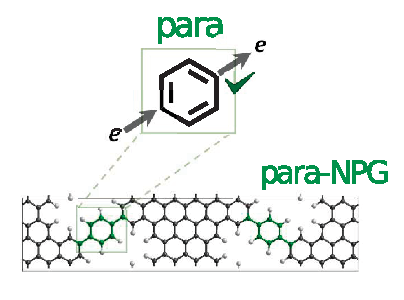
\includegraphics[width=.9\textwidth]{Figures/Parametagraphic.eps}
	    \caption{}
	    \label{Parametastructfig}
	\end{subfigure}
	\quad
	\begin{subfigure}[b]{.45\textwidth}
	    \centering
	    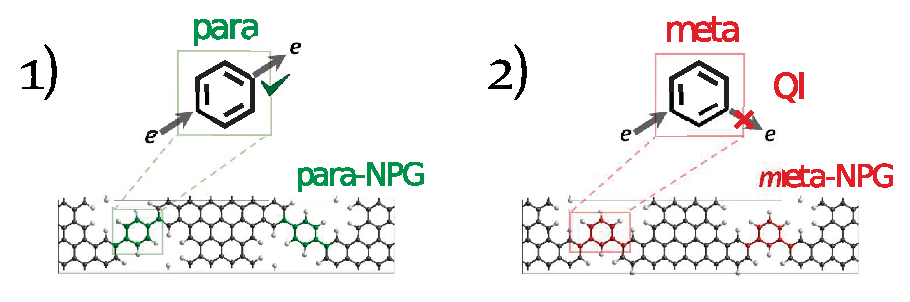
\includegraphics[width=.9\textwidth]{Figures/Metaparagraphic.eps}
	    \caption{}
    	\label{Metaparastructfig}
    \end{subfigure}
    \vskip
	\begin{subfigure}[b]{.45\textwidth}
        \centering
	    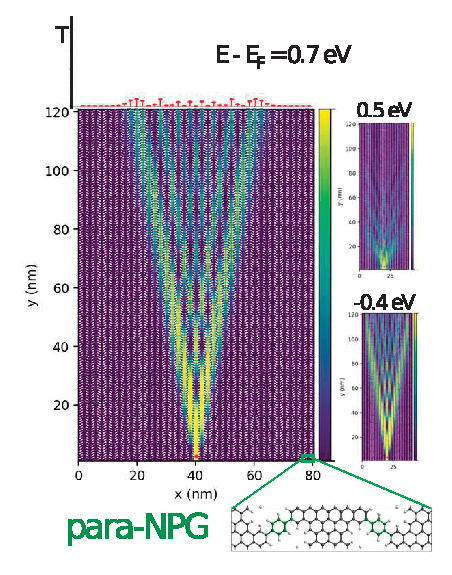
\includegraphics[width=.9\textwidth]{Figures/Fig_3para.eps}
	    \caption{}
	    \label{studyfig3para}
	\end{subfigure}
	\quad
	\begin{subfigure}[b]{.45\textwidth}
        \centering
	    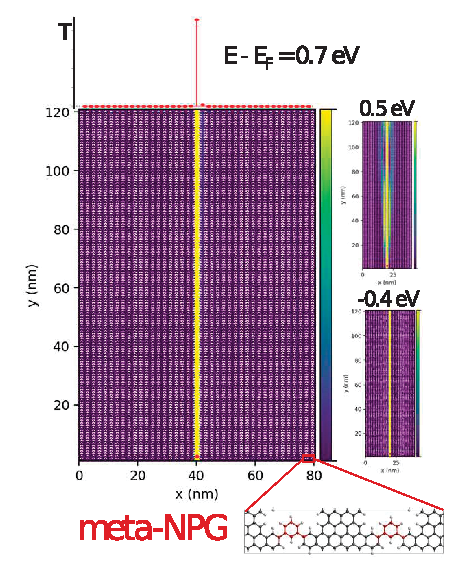
\includegraphics[width=.9\textwidth]{Figures/Fig_3meta.eps}
	    \caption{}
	    \label{studyfig3}
	\end{subfigure}
\caption{a) showing the para NPG, b) showing the meta NPG.\newline
c-d) Figures showing the currents through the GNR's in a large peace of NPG. Note how the current is spread across GNR's with the para bridge a) and confined to a single GNR with meta bridge c).\newline
Used with permission from Isaac Alcón Rovira.}
\label{studyfigs}
\end{figure}
\subsection{Bridge effects in para-NPG and meta-NPG}\label{metaparasection}
In broad terms the difference in the \textit{meta} and \textit{para} structures lies in the path an electron will travel through the benzene ring to get across the bridge between GNR's in NPG. In the para bridge, the path across the aromatic ring is symmetric and so the electron will pass above or below with equal phase. Since the para bridge has three bonds in each direction across the ring, the path length in the para bridge is the same on each side (See \cref{Parametastructfig}). This will cause constructive quantum interference of the states once the waves meet on the other side of the ring. For para NPG this causes electronic coupling between the GNR channels. In the meta bridge, the way across the aromatic ring is not symmetric in the sense that there is two bonds across the path below and four bonds across on the path above (See \cref{Metaparastructfig}). This will cause a shift by half a wavelength between the two paths and thus create destructive quantum interference between waves meeting on the other side of the ring. This causes electronic decoupling between GNR channels, allowing for confinement of injected currents in a single GNR channel\cite{unpub} (see \cref{studyfig3}). In \cref{metapara} band plots as well as transmission plots from the study\cite{unpub} are shown for para and meta NPG. In the band plots the two sets of valence/conduction bands around the Fermi level shows band splitting for para and interference for meta NPG. Looking at the transmission plots next to the band plots one can see there is transmission and thus coupling of the states between the GNR's for para. The area between the two peaks at \SI{0.5}{\electronvolt} and  \SI{1.2}{\electronvolt} show transport between the GNR's. In the transmission plot for meta the transmission is supressed (\cref{metapara} right). The transmission plot the area between the two peaks is now pretty much 0. This means GNR's are electrically decoupled in meta system. To summarise these results qualitatively: Splitting of the bands in the band plots, corresponds to effective coupling of the GNR's. Bands on top of each other, showing QI, corresponds to decoupling of the GNR's and thus electric confinement of injected currents on NPG in single GNR channels (see \cref{studyfig3}). In the following sections, band plots will mainly be used to show results. Therefore one should keep in mind how the band structures, qualitatively, relate to transmission. In \cref{appfigs}, \cref{allbands} a figure obtained from the developed functions with band plots of normal, para and meta NPG can be seen.
\begin{figure}[ht]
	\centering
	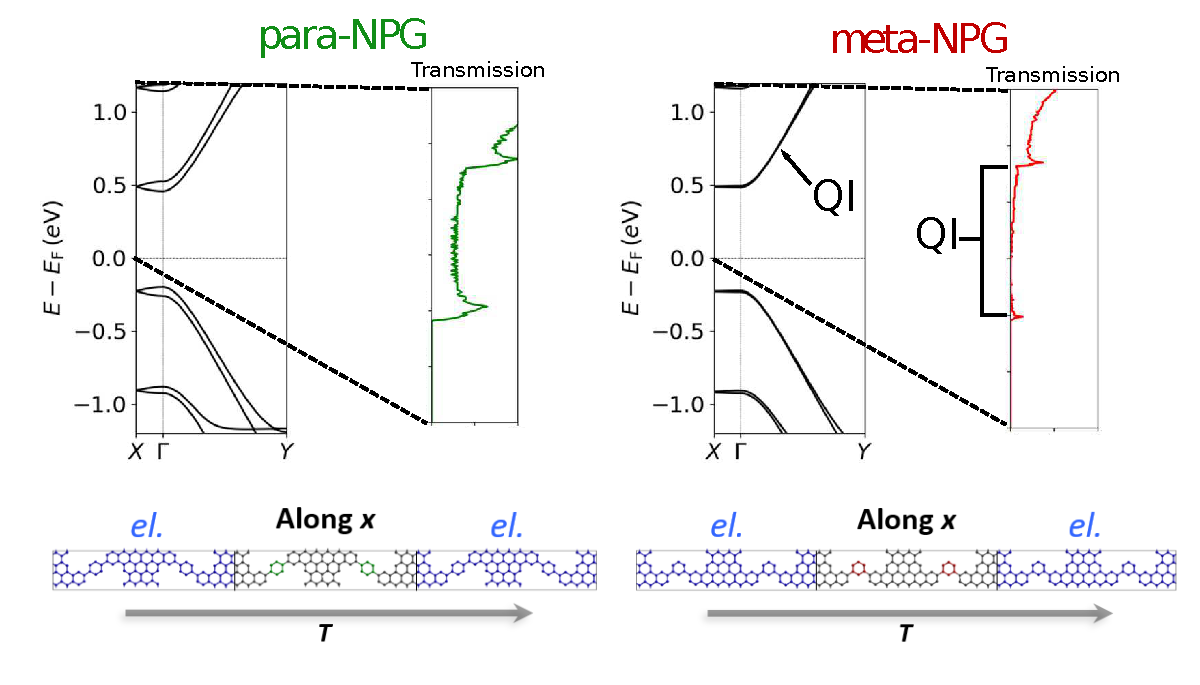
\includegraphics[width=0.8\textwidth]{Figures/metapararesultdraft.eps}
	\caption{Figure showing band plots and transmission plots for para and meta NPG. In the bottom of each plot is a schematic showing which way the transmission occurs in relation to the NPG.\newline
	Used with permission from Isaac Alcón Rovira}
	\label{metapara}
\end{figure}
\newpage
\subsection{Tests with oxygen modified meta and para-NPGs}\label{testintroduc}
The tests consist of two kinds of chemical modification. Firstly it will be bonding oxygen sites to the meta and para NPG (Addition of Oxygen will be simulated by addition of another carbon site to the structure, effectively adding another pi-electron). Secondly simulations of hydrogenation will be done by bonding hydroxide groups to the bridges. These modifications will be carried out separately. Because of the complex nature of DFT the band plots obtained via DFT makes it hard to interpret what is actually going on in the system chemically. Therefore the aim is to show that using the methods developed, based on tight-binding models, it is possible to reproduce bands structures calculated from DFT. If successful, it will provide a much easier way to understand the effect of the implemented chemical modification compared to the DFT approach. Band plots, as well as some on-site potential maps, calculated with DFT has been provided by supervisor Isaac Alcón Rovira for comparison. The geometries, used for calculations, are provided by supervisor Isaac Alcón Rovira and have been optimised by DFT using the SIESTA package\cite{Soler_2002} and the PBE functional\cite{perdew1996a}.
\subsection{Test 1: Para-O\mathinhead{_4}{_4}-NPG}\label{test1}
The first test is considering the Para-O\(_4\)-NPG. The basic structure is para-NPG where 4 oxygen sites are bonded, two on each benzene ring (See \cref{PS4OOW} ). Starting by looking at the resulting DFT plot in \cref{PS4ODFT} the first thing to notice is that the valence bands show QI and thus decouples the GNR's. So in spite having a para bridge, which normally gives coupling, decoupling occurs when oxygen is bonded to the bridges. Our first assumption to simulate the effect of such oxygen functionalisation is to add those atoms as active \(p_z\)-orbitals in our pi-conjugated system, using the standard parameters (i.e. as for carbon atoms - specifically the on-site potential and hopping value). As a baseline the potential of these atoms are thus the same. Moreover, the hydrogen, included in the provided optimised geometries, will be removed before any calculations take place. In \cref{PS4Odevnomod} one can see the resulting band structure plot, using such and electronic model and the DFT optimized structure. The band plot does not show much resemblance with the one obtained, using DFT. It is pretty much symmetric around the Fermi level and it is hard to make out whether there is coupling or decoupling between GNR's, based on the reasoning discussed in \cref{metaparasection}. Taking a look at the DFT-calculated potential map of \cref{potmapPS4O}, the sites where the oxygen is bonded, have a potential much different from that of the rest of the system (the four dark blue spots). As mentioned, the baseline of the method does not take into account differentiating on-site potentials within a cell. So to compensate for this, the on-site potential of the four bonded oxygen is changed. In \cref{PS4Odevmod} one can see the resulting band plot after the on-site potential of the bonded oxygen has been changed to \SI{-0.50}{\electronvolt}. The resulting band plot resembles the DFT calculations much more. There is now QI in the valence bands which means decoupling of the GNR's. To summarise the results the tests showed significant qualitative agreement with the DFT calculation. This helps to uncover the main effect of functionalisation of para-NPG with oxygen. Knowing that the added \(p_z\) electrons where participating in the pi-conjugated system, those orbitals had to be accounted for in the developed model by addition of extra sites. However, to qualitatively reproduce the DFT results, the on-site potential of those extra sites had to be lowered by \SI{-0.5}{\electronvolt}. This helped to explain why functionalisation with oxygen only affects the valence band of NPG and not the conduction band. In addition the developed method also reproduced the flat bands seen around the Fermi level in the DFT calculation (The developed method showed bands exactly at the Fermi level). In broad terms, these bands are related to benzene bridge in the NPG, but they originate because of the presence of the bonded oxygen. The oxygen do have an dispersive effect on the valence electrons of NPG, but they also seem to be localised in nature, which is why the flat bands occur.   
\begin{figure}[H]
	\centering
	\begin{subfigure}[b]{0.8\textwidth}
		\centering
		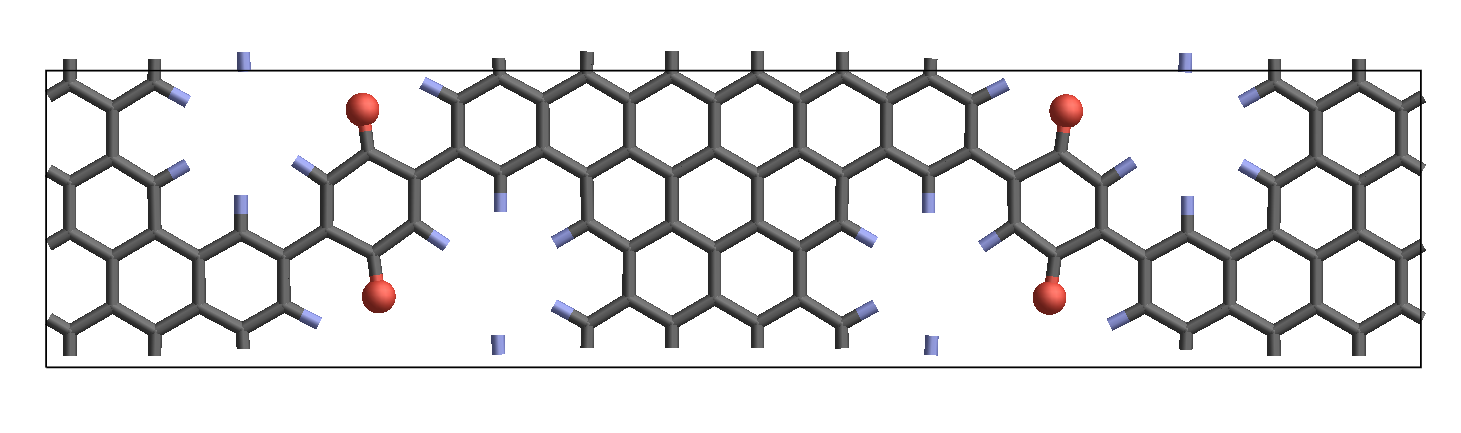
\includegraphics[width=0.8\textwidth]{Figures/para_O4.png}
		\vspace{-1\baselineskip}
		\caption{}
		\label{PS4OOW}
	\end{subfigure}
	\vskip
	\begin{subfigure}[b]{0.3\textwidth}
		\centering
		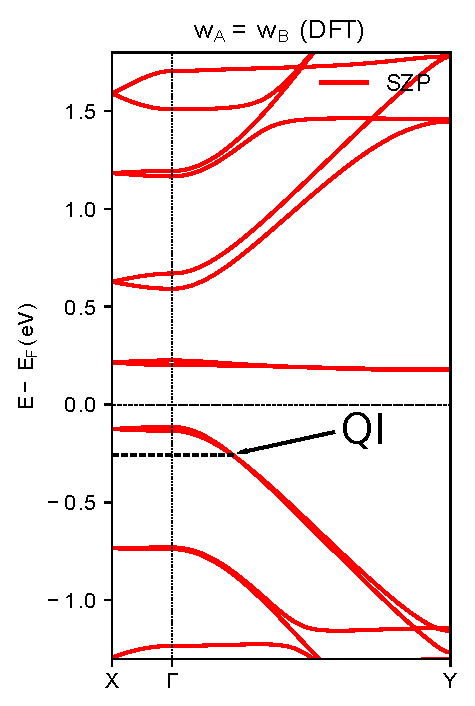
\includegraphics[width=0.8\textwidth]{Figures/PS4ODFT.eps}
		\vspace{-1\baselineskip}
		\caption{}
		\label{PS4ODFT}
	\end{subfigure}
	\hspace{-20pt}
	\begin{subfigure}[b]{0.3\textwidth}
		\centering
		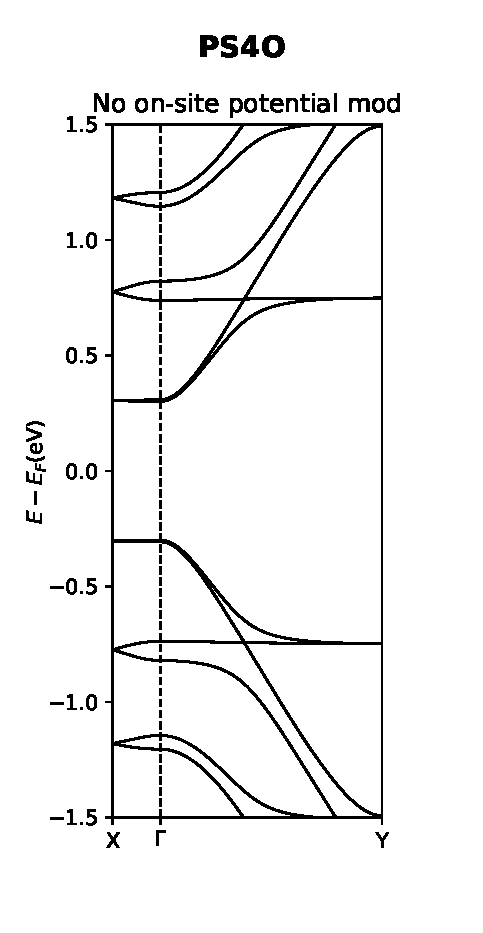
\includegraphics[width=0.8\textwidth]{Figures/PS4Onomod.eps}
		\vspace{-2\baselineskip}
		\caption{}
		\label{PS4Odevnomod}
	\end{subfigure}
	\hspace{-30pt}
	\begin{subfigure}[b]{0.3\textwidth}
		\centering
		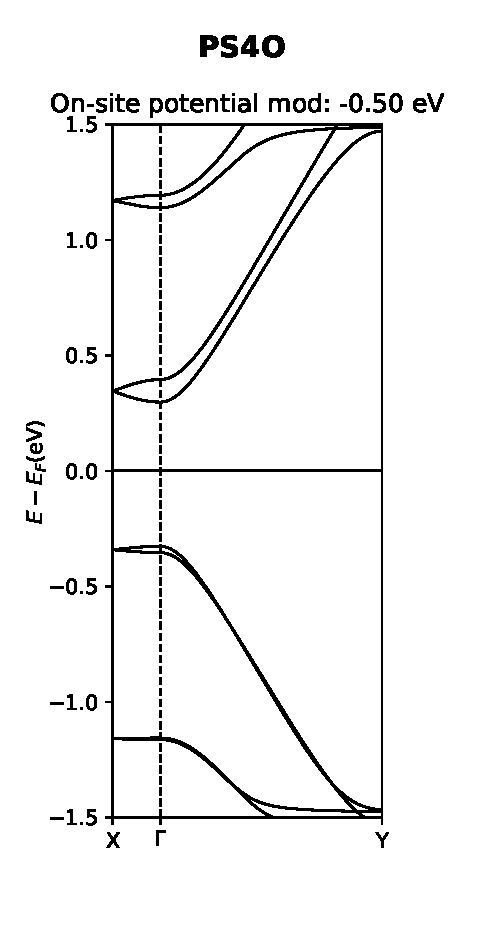
\includegraphics[width=0.8\textwidth]{Figures/PS4Omod.eps}
		\vspace{-2\baselineskip}
		\caption{}
		\label{PS4Odevmod}
	\end{subfigure}
	\vskip
	\begin{subfigure}[b]{0.8\textwidth}
	    \hspace{50pt}
		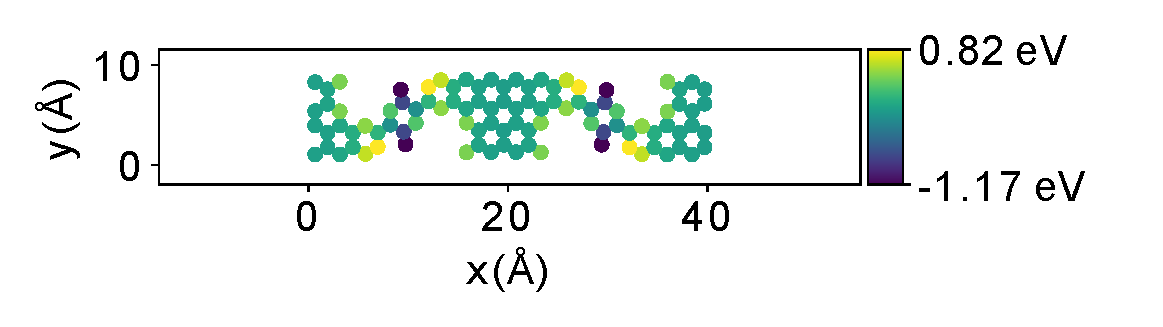
\includegraphics[width=0.8\textwidth]{Figures/PS4O.eps}
		\vspace{-0.5\baselineskip}
		\caption{}
		\label{potmapPS4O}
	\end{subfigure}
	\caption{a) Overview of the system with carbon (grey), oxygen (red) and hydrogen atoms (blue) and highlighting the added oxygen or hydroxide groups as spheres. b) Band structure obtained using DFT. c) Band structures obtained using developed program with no on-site potential mods. c) Band structures obtained using developed method with the on-site potential changed to \SI{-0.5}{\electronvolt}. d). Potential map of the system.}
	\label{PS4O}
\end{figure}
\subsection{Test 2: Para-(OH)\mathinhead{_4}{_4}-NPG}\label{test2}
Next test will be with the Para-(OH)\(_4\)-NPG system. Again the basic structure is para-NPG with bonded oxygen, but here the aim is to simulate hydrogenation, so therefore the oxygen atoms added will become hydroxide groups (See \cref{PS4OHOW}). The DFT plot in \cref{PS4OHDFT} shows a band splitting in the valence/conduction bands, so the GNR's have been coupled again. Here the first approach is to use the successfully method reproducing the DFT results in \cref{test1}: i.e. considering oxygen positions as active \(p_z\) orbitals in our model, but lowering their energy by \SI{-0.5}{\electronvolt}. In \cref{PS4OHmod2} the resulting band plot can be seen. It shows exactly the same as \cref{PS4Odevmod}. The result does therefore not resemble that of the DFT in \cref{PS4OHDFT}, which in turn is very similar to that of the pristine para-NPG (see \cref{metapara} left panel). Looking at the potential map in \cref{potmapPS4OH} it can be seen that the bonded oxygen are shifted by approximately \SI{2}{\electronvolt} down in energy with respect to the GNR's carbon atoms. Using the potential plot in \cref{potmapPS4OH} as a guide the on-sites of the oxygen are changed to \SI{-2}{\electronvolt}. The resulting plot can be seen in \cref{PS4OHdevmod}. The plot show good agreement with the DFT. The bands have split again and the GNR's are coupled. This means hydrogenation decouples the oxygen from the GNR's pi-conjugated system, so by lowering the on-site potential of one can get effective decoupling of oxygen. As seen this gives a satisfying result. Now that it is known that hydrogenation decouples the oxygen, a last hypothesis is that by simply not considering the oxygen atoms in our model the result will be similar to \cref{PS4OHdevmod}. In \cref{PS4OHremove} the resulting plot can be seen. As hypothesised, the resulting band plot show resemblance with both the DFT and \cref{PS4OHdevmod}. So the decoupling of oxygen by hydrogenation can be simulated simply by removing the hydroxide group entirely. Again there is split in the bands and thus coupling of the GNR's. This means that the developed method can uncover what happens chemically when the NPG is hydrogenated and it can do so in a simple manner.
\begin{figure}[H]
	\centering
	\begin{subfigure}[b]{0.8\textwidth}
		\centering
		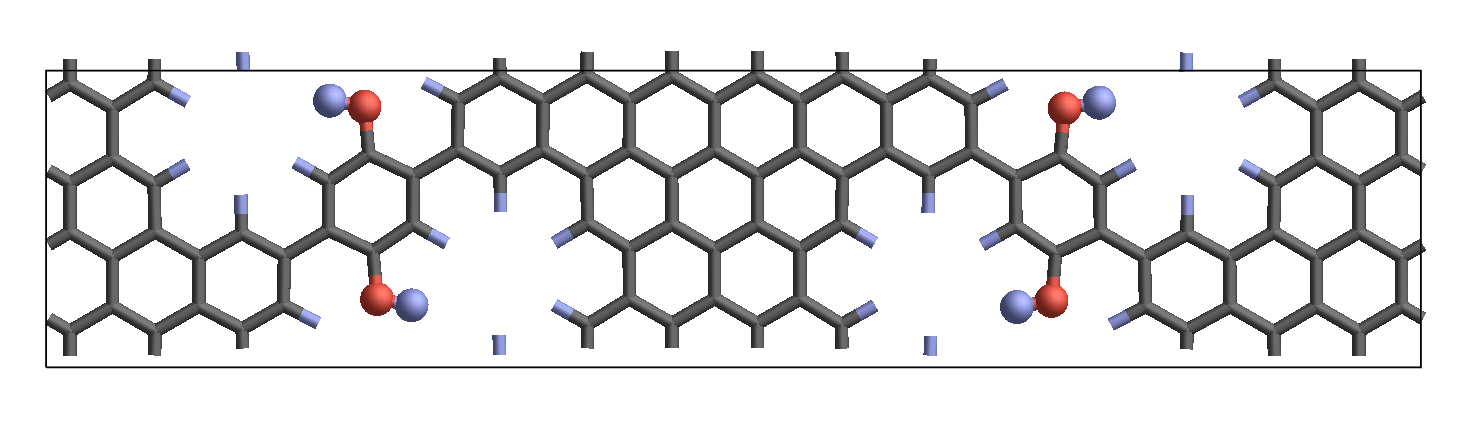
\includegraphics[width=0.8\textwidth]{Figures/para_OH4.png}
		\vspace{-1\baselineskip}
		\caption{}
		\label{PS4OHOW}
	\end{subfigure}
	\vskip
	\begin{subfigure}[b]{0.25\textwidth}
		\centering\hspace{-20pt}
		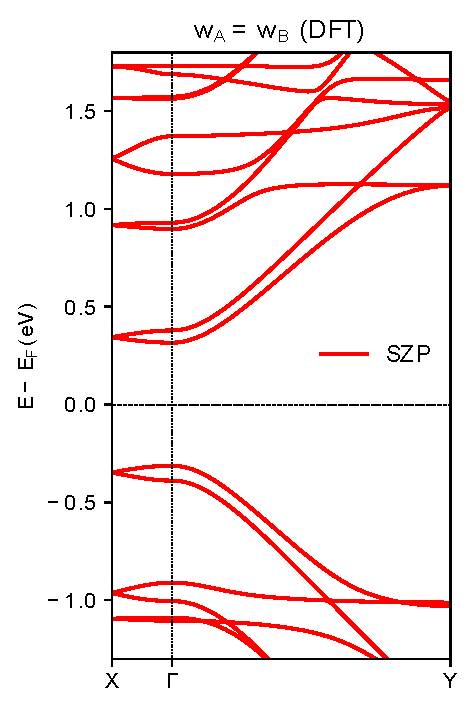
\includegraphics[width=0.8\textwidth]{Figures/PS4OHDFT.eps}
		\vspace{-1\baselineskip}
		\caption{}
		\label{PS4OHDFT}
	\end{subfigure}
	\hspace{-20pt}
	\begin{subfigure}[b]{0.25\textwidth}
		\centering
		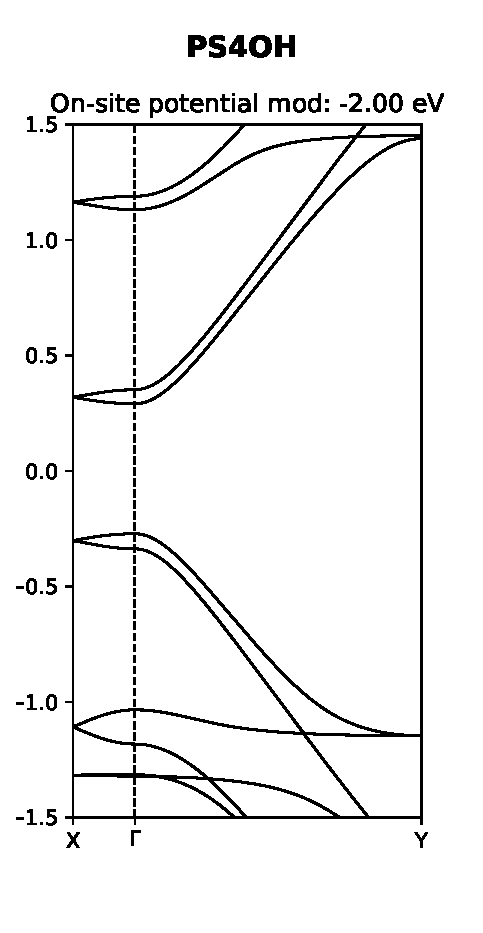
\includegraphics[width=0.8\textwidth]{Figures/PS4OHmod2.eps}
		\vspace{-2\baselineskip}
		\caption{}
		\label{PS4OHmod2}
	\end{subfigure}
	\hspace{-20pt}
	\begin{subfigure}[b]{0.25\textwidth}
		\centering
		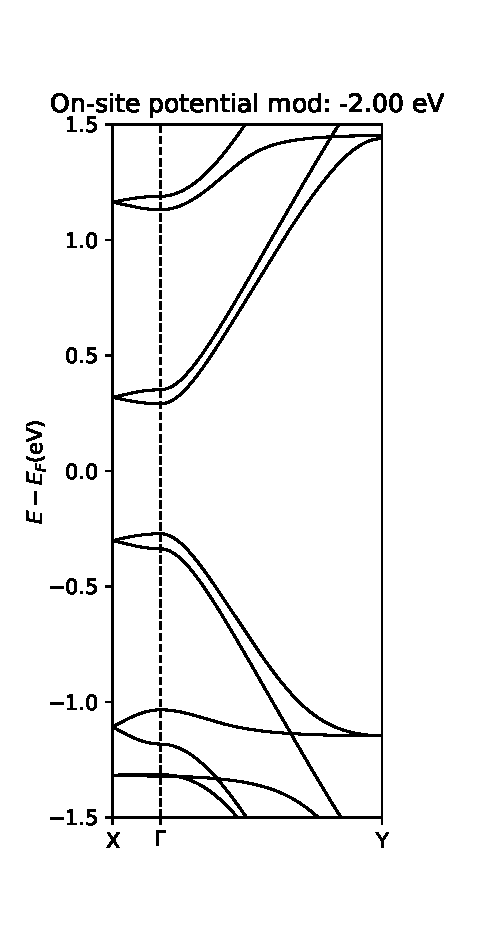
\includegraphics[width=0.8\textwidth]{Figures/PS4OHmod.eps}
		\vspace{-2\baselineskip}
		\caption{}
		\label{PS4OHdevmod}
	\end{subfigure}
	\hspace{-20pt}
	\begin{subfigure}[b]{0.25\textwidth}
		\centering
		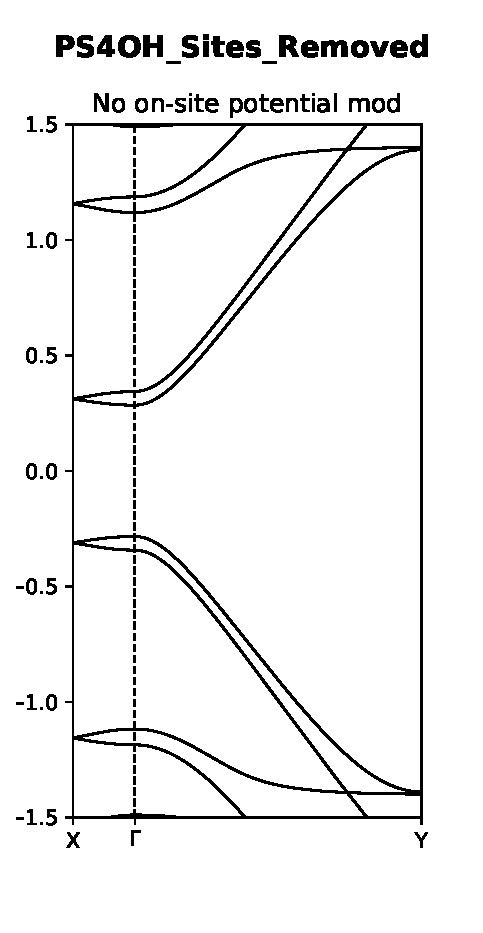
\includegraphics[width=0.8\textwidth]{Figures/PS4OHSitesRemoved.eps}
		\vspace{-2\baselineskip}
		\caption{}
		\label{PS4OHremove}
	\end{subfigure}
	\vskip
	\begin{subfigure}[b]{0.8\textwidth}
		\centering\hspace{30pt}
		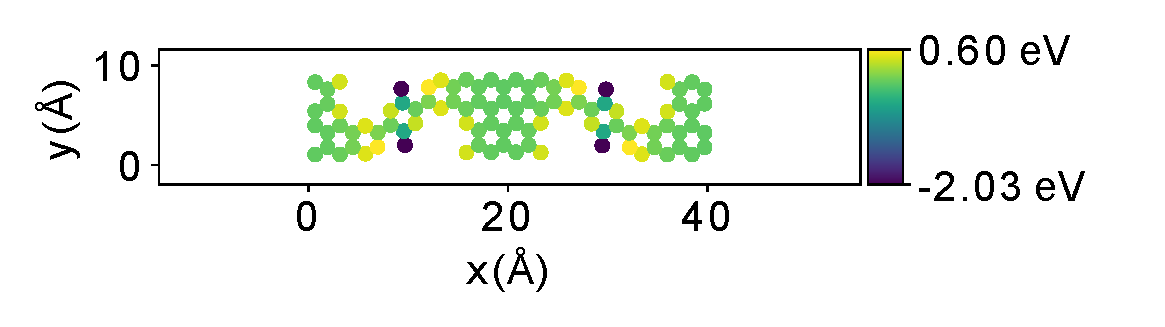
\includegraphics[width=0.8\textwidth]{Figures/PS4OH.eps}
		\vspace{-0.5\baselineskip}
		\caption{}
		\label{potmapPS4OH}
	\end{subfigure}
	\caption{a) Overview of the system with carbon (grey), oxygen (red) and hydrogen atoms (blue) and highlighting the added oxygen or hydroxide groups as spheres. b) Band structure obtained using DFT. c) Band structures obtained using developed program with with on-site potential changed to \SI{-0.5}{\electronvolt}. d) Band structures obtained using developed method with on-site potential changed to \SI{-2}{\electronvolt}. e) Band structures obtained using the developed method with sites removed. f) Potential map of the system.}
	\label{PS4OH}
\end{figure}
\subsection{Test 3: Meta-O\mathinhead{_2}{_2}-NPG}\label{test3}
Moving on to the meta NPG, the test is going to be exactly the same as \cref{test1}. To see the structure of the system look in \cref{MS2OOW}. Recall from \cref{metaparasection} that the meta NPG gives rise to QI and thus decoupling of the GNR's. However as seen in \cref{test1}, functionalising the bridges with oxygen caused some quantum interference in the para and thus decoupling of the GNR's in para NPG. Therefore one should expect some effect as well for the meta connected NPG. First the DFT plot in \cref{MS2ODFT} show that there is indeed band splitting for the valence states. Here one can also see shifts in the valence and conduction bands. The split is bigger in the valence band compared to the conduction band. So by functionalising with oxygen the effect is most prevalent at the valence band for both para and meta. Following the rationale of \cref{testintroduc}, we first consider the effect of oxygen atoms incluing them as active \(p_z\) orbitals in our mode, but with the same on-site energy value as the rest of the sites. As seen in \cref{MS2Odevnomod} we may see band splitting for both valence and conduction states. However, the plot is totally symmetric around 0 so it is not entirely accurate. Again the potential map in \cref{potmapM2SO} is used to get the on-site potential of the oxygen, so that they can be modified with the developed method. The result is seen \cref{MS2Odevmod}. Now the band plot shows split of the bands downwards, just like the DFT and the valence bands have a bigger split compared to the conduction bands. So effectively the GNR's are coupled. Now the flat bands  at the Fermi level in \cref{MS2Odevnomod} are associated with the benzene rings and they arise because of the oxygen functionalisation (i.e. they are not present in pristine meta-NPG). When the on-site potential of \SI{-0.2}{\electronvolt} is applied in \cref{MS2Odevmod} the result is in remarkably good agreement with the DFT calculations. The shape of the bands when applying the on-site potential, indicates that they are slightly more dispersive than those of \cref{PS4ODFT,PS4Odevmod}. 
\begin{figure}[H]
	\centering
	\begin{subfigure}[b]{0.8\textwidth}
	    \centering
		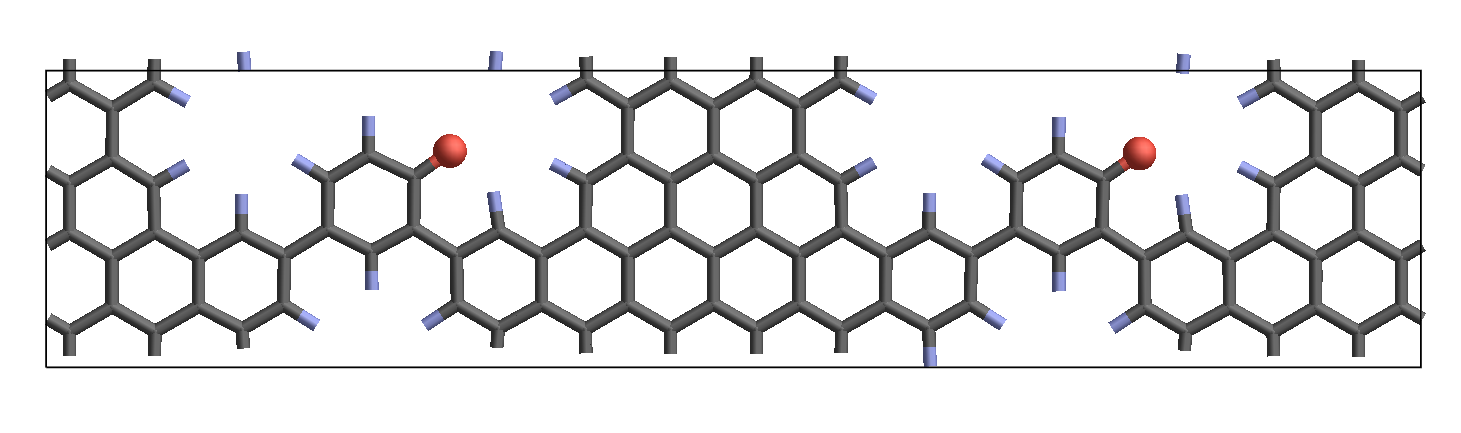
\includegraphics[width=0.8\textwidth]{Figures/meta_O4.png}
		\vspace{-1\baselineskip}
		\caption{}
		\label{MS2OOW}
	\end{subfigure}
	\vskip
	\begin{subfigure}[b]{0.3\textwidth}
		\centering
		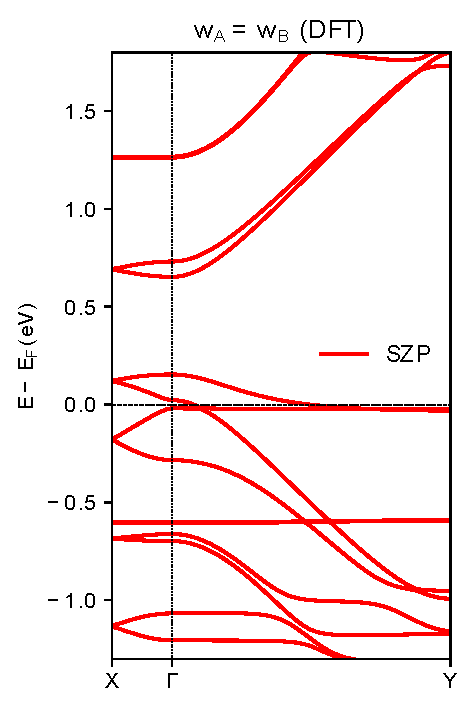
\includegraphics[width=0.8\textwidth]{Figures/MS2ODFT.eps}
		\vspace{-1\baselineskip}
		\caption{}
		\label{MS2ODFT}
	\end{subfigure}
	\hspace{-20pt}
	\begin{subfigure}[b]{0.3\textwidth}
		\centering
		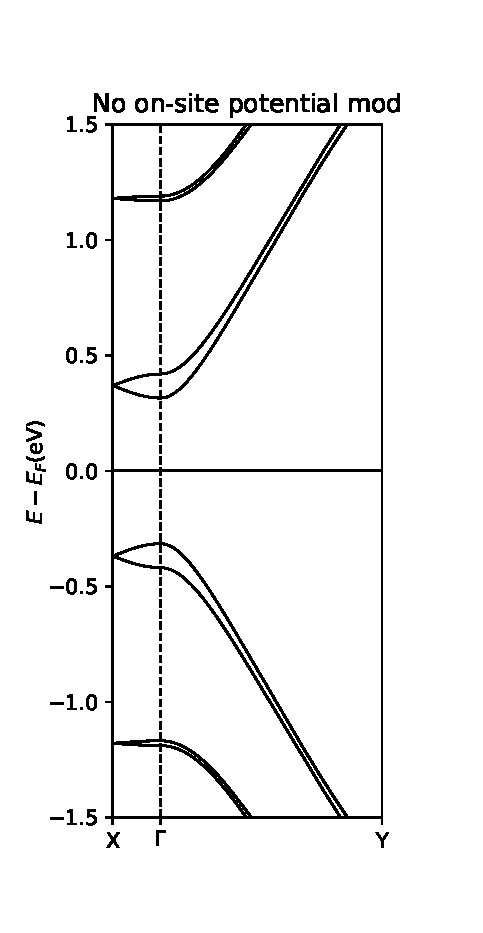
\includegraphics[width=0.8\textwidth]{Figures/MS2Onomod.eps}
		\vspace{-2\baselineskip}
		\caption{}
		\label{MS2Odevnomod}
	\end{subfigure}
	\hspace{-30pt}
	\begin{subfigure}[b]{0.3\textwidth}
		\centering
		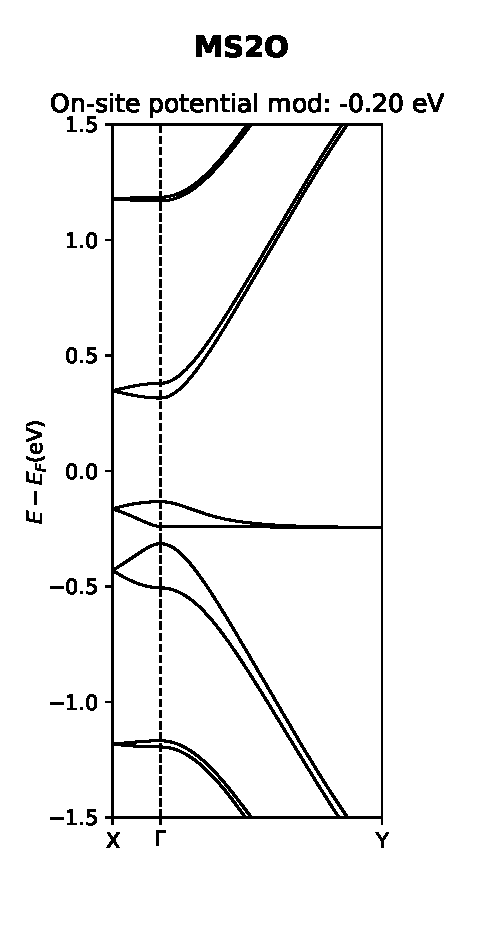
\includegraphics[width=0.8\textwidth]{Figures/MS2Omod.eps}
		\vspace{-2\baselineskip}
		\caption{}
		\label{MS2Odevmod}
	\end{subfigure}
	\vskip
	\begin{subfigure}[b]{0.8\textwidth}
	    \hspace{50pt}
		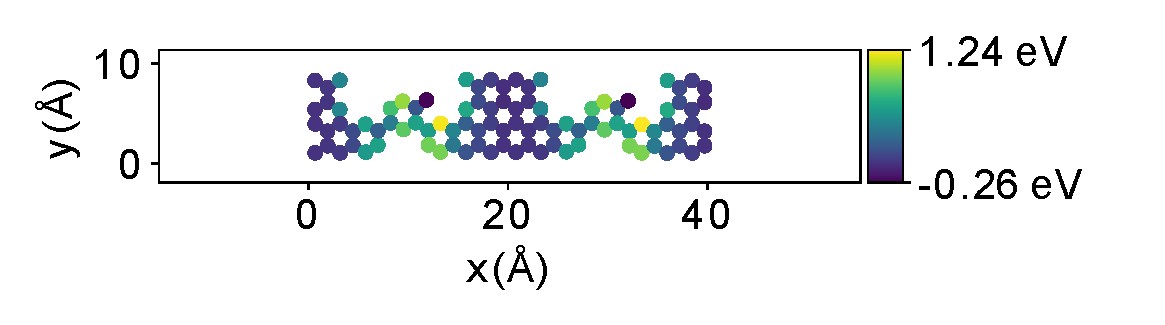
\includegraphics[width=0.8\textwidth]{Figures/MS2Opotmap.eps}
		\vspace{-0.5\baselineskip}
		\caption{}
		\label{potmapM2SO}
	\end{subfigure}
	\caption{a) Overview of the system with carbon (grey), oxygen (red) and hydrogen atoms (blue) and highlighting the added oxygen or hydroxide groups as spheres. b) Band structure obtained using DFT. c) Band structures obtained using developed program with no on-site potential mods. c) Band structures obtained using developed method with on-site potential changed to \SI{-0.2}{\electronvolt}. d) Potential map of the system.}
	\label{MS2O}
\end{figure}
\subsection{Test 4: Meta-(OH)\mathinhead{_2}{_2}-NPG}\label{test4}
The fourth and final test will be with the same approach as \cref{test2} only here the hydrogenation is of the meta-NPG with oxygen bonded. (See \cref{MS2OHOW}). The DFT plot in \cref{MS2OHDFT} shows QI for both valence and conduction bands. It is known from the para-NPG functionalised cases that hydrogen decouples the oxygen atoms from the GNR's pi-conjugated system by lowering their energy with respect to the carbon system. In \cref{potmapMS2OH} one can see that this is indeed the case. The on-site value of the bonded oxygen is much lower than that of the carbon atoms. Therefore we try to model the system by considering the oxygen atoms and lowering their the on-site potentials according to the potential map in \cref{potmapMS2OH}} fact. The resulting band plot can be seen in \cref{ms2ohdevmod}. The plot is in good agreement with DFT, showing effective decoupling of oxygen and thus decoupling of GNR's just like the unmodified meta NPG discussed in \cref{metaparasection}. Finally by removing the hydroxide group entirely, using the developed method afterwards, the resulting band plot in \cref{MS2OHremove} is obtained. The result is also in good agreement with DFT. This again proves that the developed method can uncover the chemical effects of functionalisation with oxygen and subsequent hydrogenation in a simple manner.
\begin{figure}[H]
	\centering
	\begin{subfigure}[b]{0.8\textwidth}
		\centering
		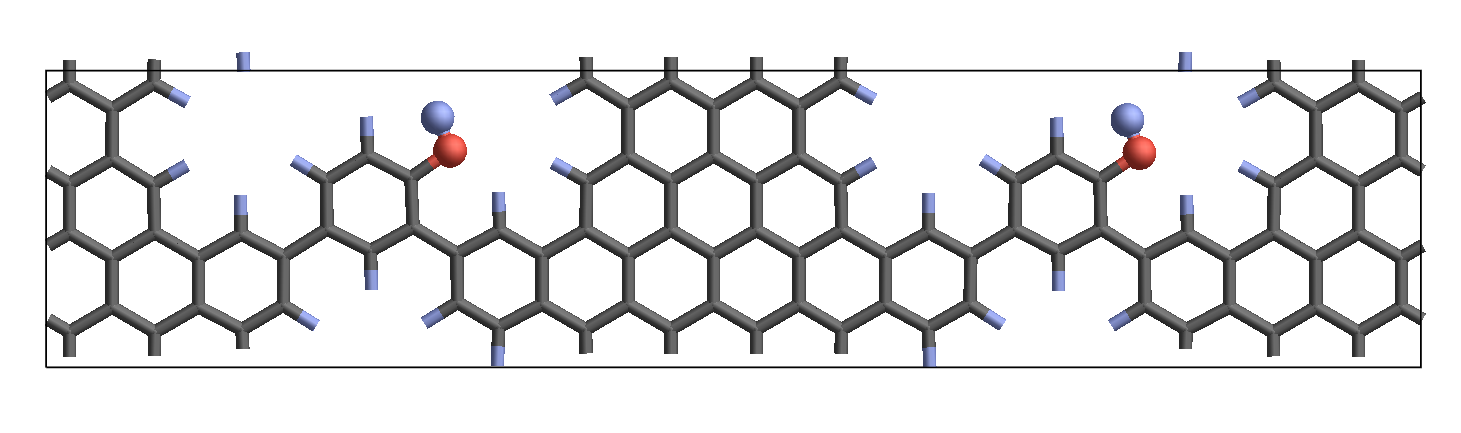
\includegraphics[width=0.8\textwidth]{Figures/meta_OH4.png}
		\vspace{-1\baselineskip}
		\caption{}
		\label{MS2OHOW}
	\end{subfigure}
	\vskip
	\begin{subfigure}[b]{0.25\textwidth}
		\centering
		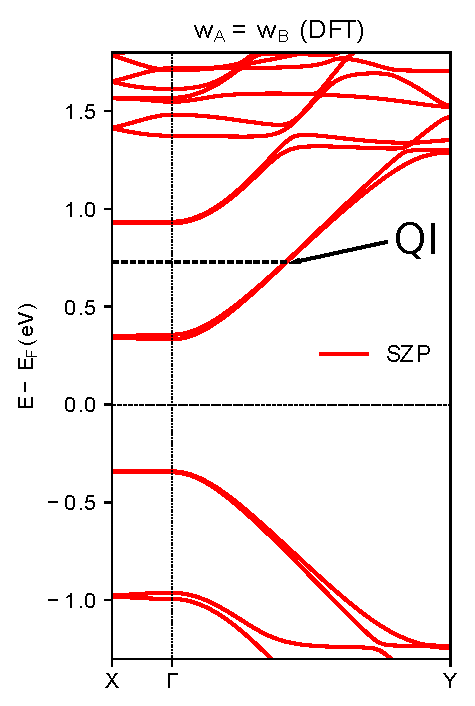
\includegraphics[width=0.8\textwidth]{Figures/MS2OHDFT.eps}
		\vspace{-1\baselineskip}
		\caption{}
		\label{MS2OHDFT}
	\end{subfigure}
	\hspace{-20pt}
	\begin{subfigure}[b]{0.25\textwidth}
		\centering
		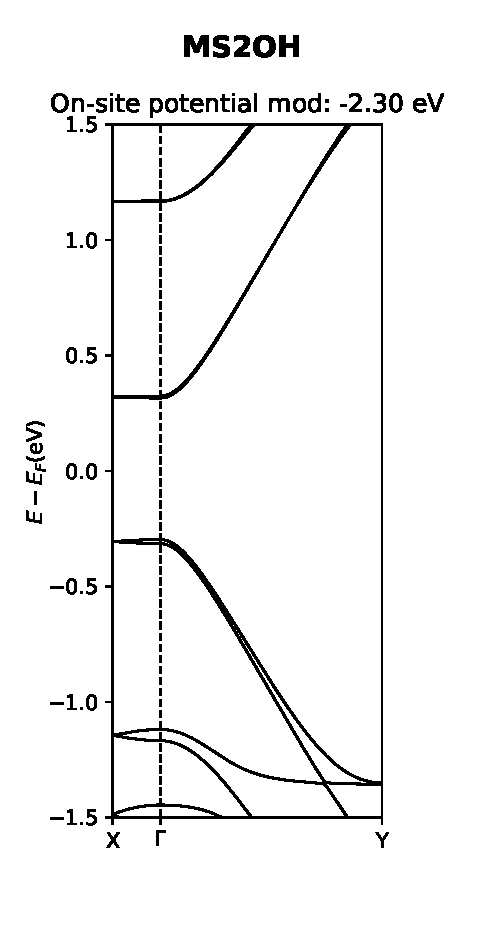
\includegraphics[width=0.8\textwidth]{Figures/MS2OHmod2.eps}
		\vspace{-2\baselineskip}
		\caption{}
		\label{MS2OHdevmod2}
	\end{subfigure}
	\hspace{-20pt}
	\begin{subfigure}[b]{0.25\textwidth}
		\centering
		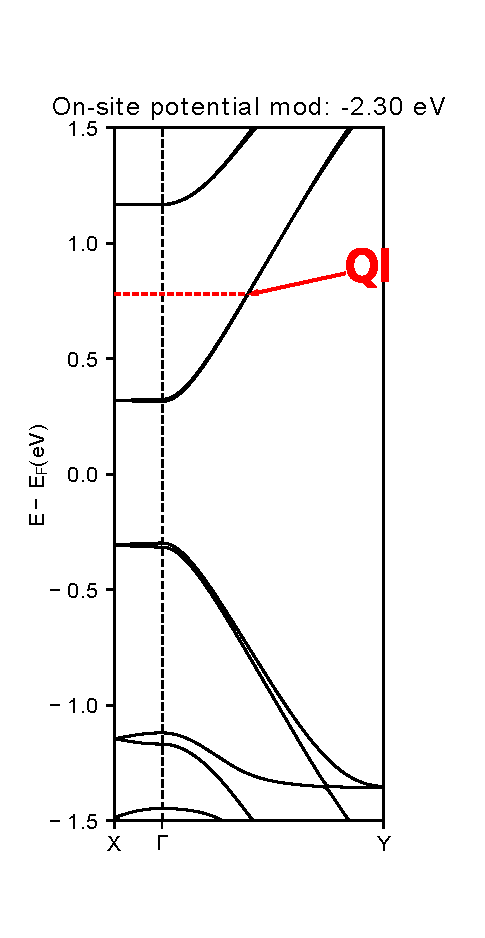
\includegraphics[width=0.8\textwidth]{Figures/MS2OHmod.eps}
		\vspace{-2\baselineskip}
		\caption{}
		\label{MS2OHdevmod}
	\end{subfigure}
	\hspace{-20pt}
	\begin{subfigure}[b]{0.25\textwidth}
		\centering
		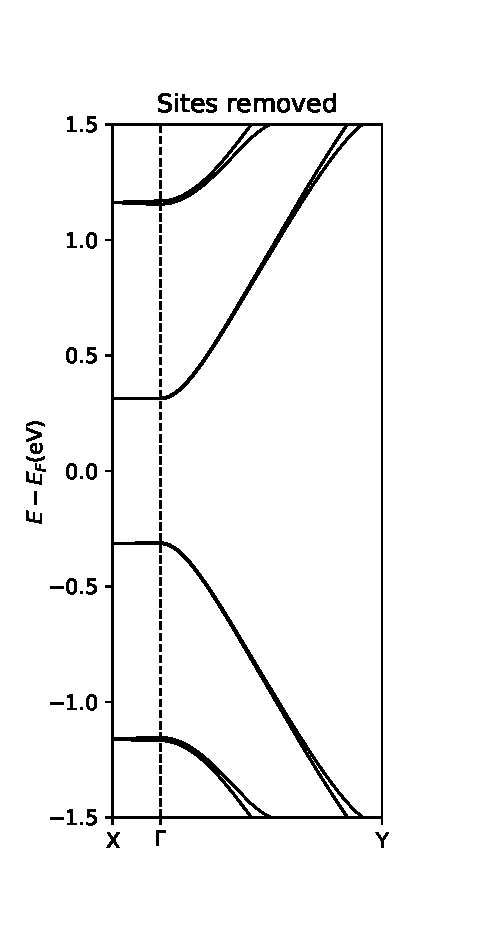
\includegraphics[width=0.8\textwidth]{Figures/MS2OHSitesRemoved.eps}
		\vspace{-2\baselineskip}
		\caption{}
		\label{MS2OHremove}
	\end{subfigure}
	\vskip
	\begin{subfigure}[b]{0.8\textwidth}
		\centering\hspace{30pt}
		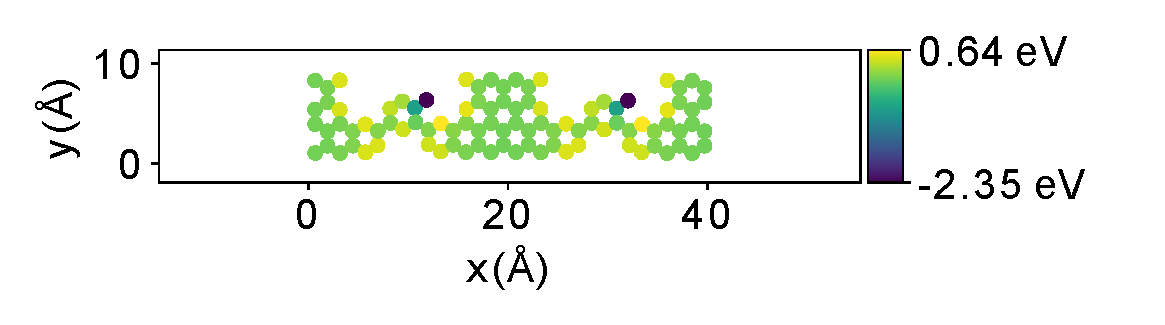
\includegraphics[width=0.8\textwidth]{Figures/MS2OH.eps}
		\vspace{-0.5\baselineskip}
		\caption{}
		\label{potmapMS2OH}
	\end{subfigure}
	\caption{a) Overview of the system with carbon (grey), oxygen (red) and hydrogen atoms (blue) and highlighting the added oxygen or hydroxide groups as spheres. b) Band structure obtained using DFT. c) Band structures obtained using developed program with with on-site potential changed to \SI{-0.2}{\electronvolt}. d) Band structures obtained using developed method with on-site potential changed to \SI{-2.3}{\electronvolt}. e) Band structures obtained using the developed method with sites removed. f) Potential map of the system.}
	\label{MS2OH}
\end{figure}
\subsection{Test summary}
For the para systems, the added oxygen introduced some QI to the system. It was possible to show that the developed program could reproduce the results obtained from DFT. This did require some adjustment to the on-site potential of the added oxygen. By hydrogenation of the oxygen it was shown that the system again returned to a shift in the bands. Again by adjusting the on-site potential it was possible to obtain results very close to the DFT calculation. The results are also comparable with the ones mentioned in \cref{metaparasection}. This shows that hydrogenation of oxygen can change the system to resemble regular para-NPG, even if it has oxygen bonded. The same can be said for the meta tests. All in all these results give a better, intuitive understanding of what happens with chemically with the systems and what effect it has on the electron transport in NPG. This is because all manipulations can be followed with ease and the results are easy to interpret. The tests have shown that it is possible to tune the electrical properties of chemically modified meta and para NPG by hydrogenation and thus providing a novel approach in designing sensitive nano circuitries, for f.ex. PH-sensors. This rounds off the summary of the test section. The section following will conclude the project as a whole.
